\documentclass[UTF8]{ctexart}
\usepackage{bookmark}
\usepackage{geometry}
\usepackage{hyperref}
\geometry{a4paper,scale=0.8}
\usepackage{ctex}
\usepackage{booktabs}
\usepackage{array}
\usepackage{fancyhdr}
\usepackage{physics}
\pagestyle{fancy}
\fancyhf{}
\renewcommand\footrulewidth{1pt}
\lhead{\textit{王铠泽}}
\rhead{\textit{PB18020766}}
\chead{\href{mailto:volar@mail.ustc.edu.cn}{\textit{volar@mail.ustc.edu.cn}}}
\rfoot{\href{http://en.ustc.edu.cn/}{\textit{中国科学技术大学}}}
\lfoot{\textit{\today}}
\usepackage{graphicx}
\usepackage{float}
\usepackage{subfigure}
\fancyfoot[C]{\textit{\thepage}}


\begin{document}

	\centering\textbf{\LARGE{计算物理A第十五次作业}}
	
	\pagenumbering{arabic}
	\textit{王铠泽\qquad PB18020766}
	
		
	\section{作业题目}
	
	\begin{itemize}
	\item	设体系的能量为 $H=x^2/2\sigma_x^2+y^2/2\sigma_y^2$
	(以$ kT $为单位),采用$ Metropolis $抽样法
	计算$\langle x^2 \rangle$,$\langle y^2 \rangle$,$\langle x^2+y^2 \rangle$
	,并与解析结果进行比较。抽样时在2维平面上依次标出Markov
	链点分布,从而形象地理解Markov链。
	\end{itemize}

	\section{实现方法和原理}
	
	\begin{itemize}
		\item $Metropolis$抽样方法
		
		本次实验中,设$\sigma_x=\sigma_y=1$
		
		理论上解析计算得到:
		
		$$\langle x^2 \rangle=\frac{1}{Z}\int_{-\infty}^\infty dy \int_{-\infty}^\infty dx\,exp\left(-\frac{x^2}{2}-\frac{y^2}{2}  \right)x^2 $$
		其中$Z$为配分函数,其数值为:
		
		$$Z=\int_{-\infty}^\infty dy \int_{-\infty}^\infty dx\,exp\left(-\frac{x^2}{2}-\frac{y^2}{2}  \right)=2\pi $$
		
		$$\Rightarrow \langle x^2 \rangle=1$$
		
		同理得到:
		
		$$\langle y^2 \rangle=1,\langle x^2+y^2 \rangle=2$$
		
		
		采用正则系统的$Boltzmann$分布作为平衡构型时的分布。所以从$(x,y)$过渡到$(x',y')$的概率为:
		
		$$p(\vec{x}\rightarrow\vec{x'})=min\{1,exp(\frac{x^2/2\sigma_x^2+y^2/2\sigma_y^2}{x'^2/2\sigma_x^2+y'^2/2\sigma_y^2})\}$$
		
		算法基本描述:
		
		本次实验采用每次在原来位置上随机抽取$[-A,A]$上的随机数作为$dx$、$dy$,进行概率判断。若能量降低,则前进概率等于1,直接进入下一个状态。若概率小于1,则再次生成$[0,1]$中的随机数$r$,若$r<exp(\frac{\Delta E}{kT})$,则刷新状态,进行下一步,否则就维持原样。
		
%			\begin{figure}[H]
%			\centering  %图片全局居中
%			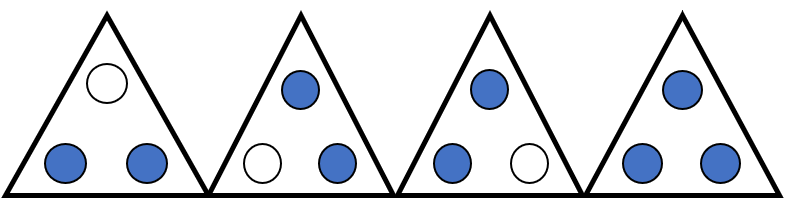
\includegraphics[width=4in]{../result/2.png}
%			\caption{导通条件(蓝色填充表示被占据)}
%		\end{figure}
%	

	最后注意:采用$Metropolis$抽样计算系综平均时要去掉热化阶段:
	
	$$\langle X \rangle=\frac{1}{N-M}\sum_{i=M+1}^{N} X_i$$
	
	
	
%	\begin{figure}[H]
%		\centering  %图片全局居中
%		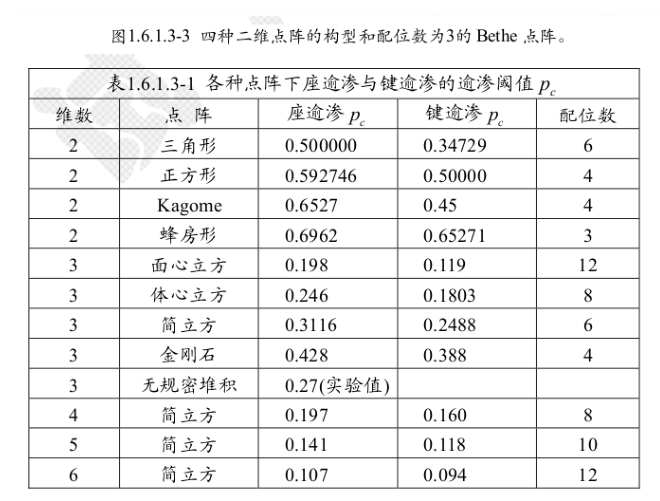
\includegraphics[width=6in]{../result/3.png}
%		\caption{正确值表}
%	\end{figure}
\end{itemize}
	
	\section{程式说明}
	
		\begin{itemize}
		\item metropolis.c
		
		这是一个对于用于生成对于$N=10^{6}$步数的$Metropolis$抽样计算积分的误差评估的程序。
	
		
		\item rdm.h
		
		这是一个包含了使用16807产生器生成指定长度的$[0,1]$上均匀分布随机数函数的头文件。
		
		\subitem void rdm(int N,double *x,int method)
		
		该函数将输入的指针$x$对应的长度为$N$的数组用$[0,1]$上的随机数填满。method是关于初始种子的选择。method=0:默认种子;method=1,时间种子。
		
		\item time\_seed(gamma range).txt
		
		对于括号内标识的$\gamma$取值范围对应使用的时间种子文件。注意在程式中生成随机数时,一组随机数使用时间种子,另一组采用默认种子值($I$=1)。16807产生器抽样时对应的时间种子数据(每次1个种子)。调用多少次16807生成器就生成多少个数据记录。每一个分布对应的种子已经手动加上对应的实验了。种子产生公式如下:
		
		
		
		\begin{figure}[H]
			\centering  %图片全局居中
			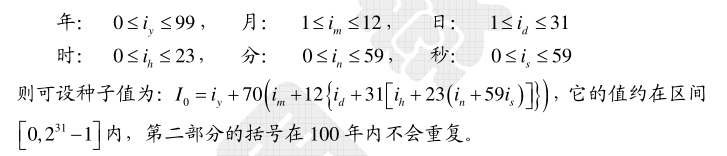
\includegraphics[width=4in]{../result/1.png}
		\end{figure}
		
	\end{itemize}
	

	\section{计算结果}
	\subsection{不同步长下的平均值计算}
	\begin{flushleft}
		本次实验中,采取总步长$N=10^6$,热化步长$M=10^4$。为了探究不同行走步长$A$对结果的影响,对其取值如下:
		
		$$A=0.001,0.002,0.005,0.01,0.04,0.08,0.1,0.5,1,2,4,10,100$$
		
		由此得到的$\langle x^2 \rangle,\langle y^2 \rangle,\langle x^2+y^2 \rangle$列表如下:
		
			\setlength{\tabcolsep}{5mm}{
			\begin{table}[H]
				\centering
				\begin{tabular}{@{}lllllll@{}}
					\toprule
					系综平均$N$&$A=0.001$&$A=0.002$&$A=0.005$&$A=0.01$&$A=0.04$&$A=0.08$ \\ \midrule
					$\langle x^2 \rangle$&59.965622&42.503714&9.911649&3.336977
					&0.916165&0.983122\\
					$\langle y^2 \rangle$&31.747700	&21.228011&4.922366&1.654147&0.899795&
				0.930838\\
					$\langle x^2+y^2 \rangle$&91.713322&63.731725&14.834015&4.991124&1.815960&1.913960\\
					\bottomrule
				\end{tabular}
				\caption{$A=0.01\sim0.08$系综平均计算表格}
		\end{table}}
	
			\setlength{\tabcolsep}{4mm}{
			\begin{table}[H]
				\centering
				\begin{tabular}{@{}llllllll@{}}
					\toprule
					系综平均$N$&$A=0.1$&$A=0.5$&$A=1$&$A=2$&$A=4$&$A=10$&$A=100$ \\ \midrule
					$\langle x^2 \rangle$&0.999358	&1.002436&1.000011&0.998231
					&1.000731&1.005191&1.049830\\
					$\langle y^2 \rangle$&0.950428	&1.010010&1.000383&0.995312&1.001040&1.001623&1.045211\\
					$\langle x^2+y^2 \rangle$&1.949786&2.012446&2.000394&1.993542&2.001770&2.006814&2.095041\\
					\bottomrule
				\end{tabular}
				\caption{$A=0.1\sim100$系综平均计算表格}
		\end{table}}
		
		从上面的表格可以看出,系综平均的计算值误差随步长并不是单调的关系。步长过小/过大都不能得到很好的结果,这将在稍后继续讨论。我们的模拟方法存在一个“最佳步长”,不至于太小,走不到理想分布;也不至于太大,每一步的涨落太大,这13个值中最佳的是$A=0.04$。下面给出$\langle x^2+y^2 \rangle$的误差表格以更加直观地表述上面的观点。
		
			\setlength{\tabcolsep}{20mm}{
			\begin{table}[H]
				\centering
				\begin{tabular}{@{}ll@{}}
					\toprule
					步长&误差$\epsilon$\\ \midrule
					$A=0.001$&89.713322\\
					$A=0.002$&61.731725\\
					$A=0.005$&12.834015\\
					$A=0.01$&2.991124\\
					{$A=0.04$}&0.184040\\
					$A=0.08$&0.086040\\
					$A=0.1$&0.050214\\
					$A=0.5$&0.012446\\
					$A=1$&0.000394\\
					$A=2$&0.006458\\
					$A=4$&0.001770\\
					$A=10$&0.006814\\
					$A=100$&0.095041\\
					\bottomrule
				\end{tabular}
				\caption{$A=0.01\sim100$系综平均误差表格}
		\end{table}}
		
		将误差-步长曲线绘制如下(由于取值范围跨度较大,取用对数坐标):
		
			\begin{figure}[H]
				\centering  %图片全局居中
				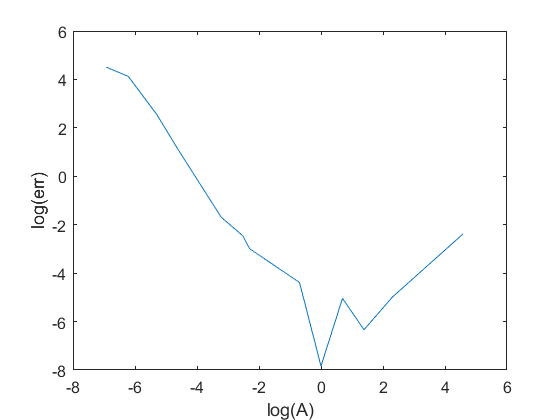
\includegraphics[width=4in]{../result/err.png}
				\caption{误差曲线}
			\end{figure}
		
	\begin{flushleft}
			\qquad显然在$A=1$附近会存在极小值,过大或过小步长误差会增大,特别是小步长。还可以从$Markov$链抽样出来的$x$最终分布的形态来观察是否达到良好的平衡构型,得到准确的结果。理论上,平衡态时,$x,y$的边缘分布都是$\sigma=1$的高斯分布。下面分别给出$A=0.001$(小步长),$A=1$(恰当步长),$A=10$(大步长),$A=100$(巨大步长)的$x$直方图统计情况。我们在下一小节中集中讨论这些问题。
	\end{flushleft}
		
		
	\section{$Markov$链的进一步讨论}
		
	\begin{flushleft}
			\begin{flushleft}
				首先给出热化之后的$x$分布直方图:
			\end{flushleft}
	
	\begin{flushleft}
		\qquad 从图上可以看出,当步长过小或者过大时分布都不是那么理想,特别是步长小的时候,就算用尽了$N=10^{6}$步,看起来似乎离平衡位置还很远。并且可以看到小步长的概率密度图上有很多个小峰状结构,这是由于步长太小,倾向于在一个地方“打转”的可能性变大了,所以出现一系列峰。	
		
		\qquad 至于在步长很大($A=100$)的时候,分布倒是已经体现出正态分布的雏形了,对称性也基本具备,但是由于步数不够多,还不够得到平衡时的理想构型。从$(b),(c),(d)$三图能明显看出分布被步长变大破坏的过程。
		
		\qquad 总的来说,步数越大越能得到理想效果;步长要选取合适的,一般判据是选取步长和数据方差在一个数量级,这样得到的收敛速度快,精度高。对于$Markov$链直观的可视化抽样图如下给出:
		
	\end{flushleft}	
			
			\begin{figure}[H]
				\centering  %图片全局居中
				\subfigure[$A=0.001$]{
					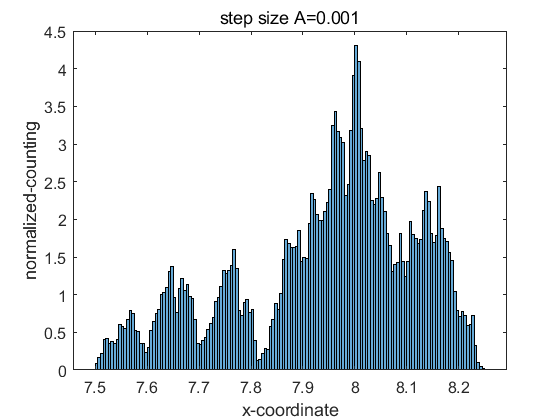
\includegraphics[width=0.45\textwidth]{../result/s_count}}
				\subfigure[$A=1$]{
					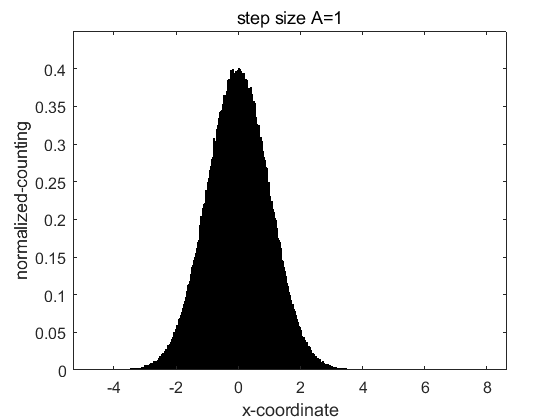
\includegraphics[width=0.45\textwidth]{../result/m_count}}
				\subfigure[$A=10$]{
					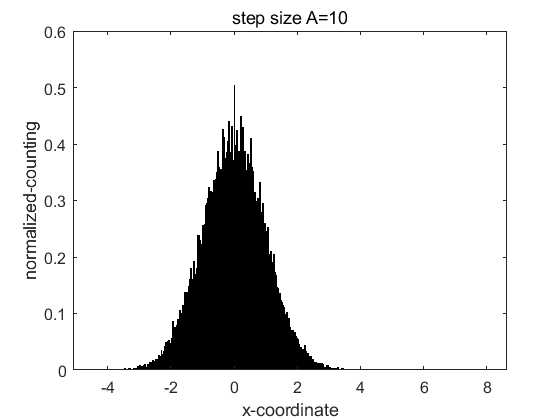
\includegraphics[width=0.45\textwidth]{../result/b_count}}
				\subfigure[$A=100$]{
					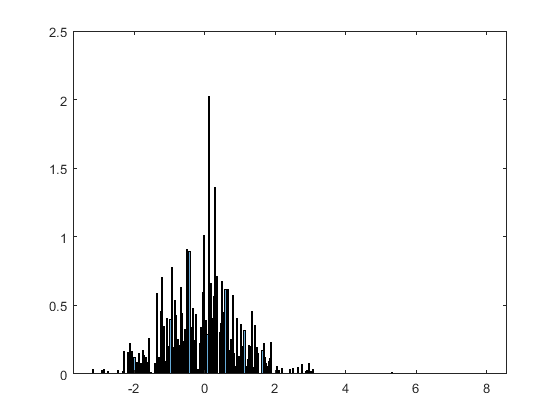
\includegraphics[width=0.45\textwidth]{../result/h_count}}
				\caption{不同$A$情况的$x$分布概率密度}
				
			\end{figure}
	\end{flushleft}
		
		
		
			\begin{figure}[H]
					\centering  %图片全局居中
					\subfigure[$A=0.001$]{
						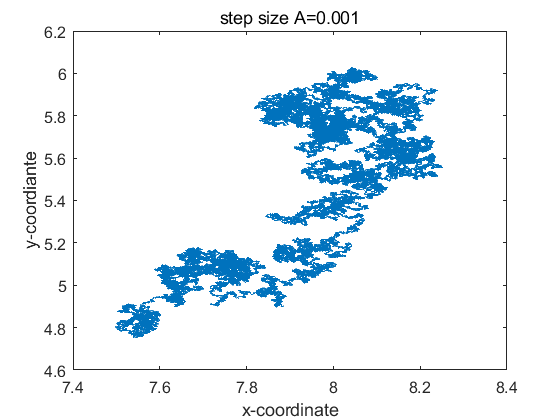
\includegraphics[width=0.45\textwidth]{../result/s}}
					\subfigure[$A=1$]{
						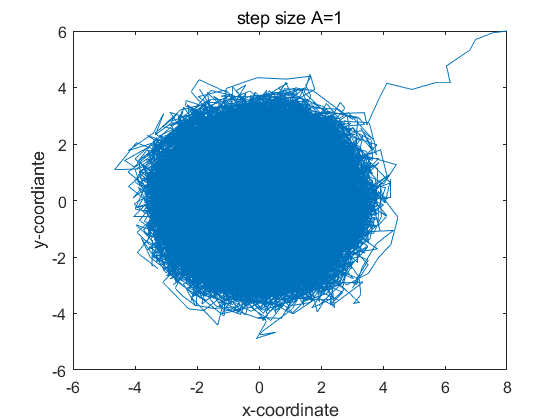
\includegraphics[width=0.45\textwidth]{../result/m}}
					\subfigure[$A=10$]{
						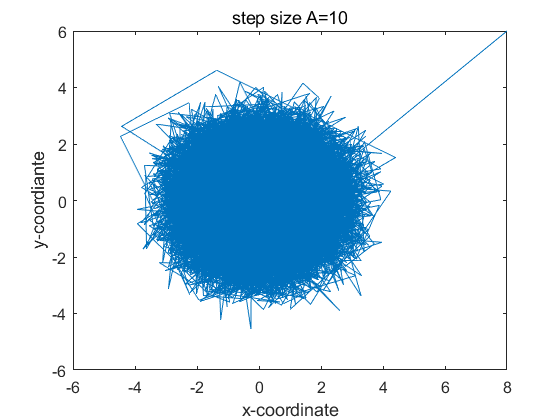
\includegraphics[width=0.45\textwidth]{../result/b}}
					\subfigure[$A=10$]{
						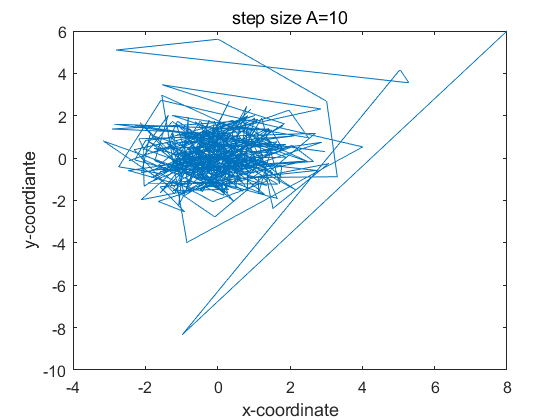
\includegraphics[width=0.45\textwidth]{../result/h}}
					\caption{不同$A$情况$Markov$链抽样情况}
					
				\end{figure}
		
		\qquad 三个$Markov$链都是从($x_0,y_0$)=(8,6)开始摸拟。在小步长$A=0.001$情况下,至循环结束时才行走到大约(7.4,4.4)处,不能有效进入理想构型附近\textbf{。此时的运动更加接近的是$Brown$运动,带有随机游走的特征}。我们可以粗略地估计一下,如果是理想的布朗运动,$\Delta x\approx \sqrt{N}A\approx1$,这和(a)图吻合得很好。而大步长下的轨迹显然比“最佳步长”的要粗糙很多,毛刺更明显,在平衡位置附近涨落更大,也不能得到理想的结果。
		
	
	
	\end{flushleft}
	
	
	
	
	
	

	\section{总结}
	\begin{itemize}
		\item $Metropolis$抽样是摸拟各种系综的一个简单直观的抽样方法,有很大的实用性。
		\item $Metropolis$抽样的缺点也很明显,非常依赖于步长(步进频率分布)的选取,有一定的预实验或者计算前的估计非常重要。
	\end{itemize}
	

\end{document}